\documentclass[10pt,a4paper]{article}
\usepackage[margin=0.75in,top=0.67in,bottom=0.67in]{geometry}
\usepackage[T1]{fontenc}
\usepackage{lmodern,microtype,graphicx,booktabs,array,multirow,amsmath,amssymb}
\usepackage{xcolor,caption,subcaption,enumitem,placeins,fancyhdr,titlesec,listings}
\usepackage[numbers,sort&compress]{natbib}
\usepackage{hyperref}
\definecolor{ink}{gray}{0}
\definecolor{teal}{gray}{0}
\definecolor{pale}{gray}{0.96}
\colorlet{linkblue}{blue!50!black}
\hypersetup{colorlinks=true,linkcolor=linkblue,citecolor=linkblue,urlcolor=linkblue,filecolor=linkblue,pdftitle={Counting, Hashing and Scale: A Comparative Study of Seven Approximate Membership Filters},pdfauthor={CS-301 Project Group, IIT Ropar}}
\captionsetup{font=small,labelfont=bf,skip=5pt}
\setlength{\parindent}{0pt}
\setlength{\parskip}{4pt plus 1pt}
\clubpenalty=10000
\widowpenalty=10000
\setlength{\textfloatsep}{11pt plus 2pt minus 2pt}
\setlength{\intextsep}{10pt plus 2pt minus 2pt}
\newcolumntype{L}[1]{>{\raggedright\arraybackslash}p{#1}}
\renewcommand{\arraystretch}{1.15}
\titleformat{\section}{\large\bfseries\color{ink}}{\thesection}{0.65em}{}
\titleformat{\subsection}{\normalsize\bfseries}{\thesubsection}{0.65em}{}
\titlespacing*{\section}{0pt}{10pt}{5pt}
\titlespacing*{\subsection}{0pt}{7pt}{3pt}
\setlist[itemize]{leftmargin=1.35em,itemsep=2pt,topsep=3pt,parsep=0pt}
\setlist[enumerate]{leftmargin=1.6em,itemsep=2pt,topsep=3pt,parsep=0pt}
\lstset{basicstyle=\ttfamily\footnotesize,backgroundcolor=\color{pale},frame=single,rulecolor=\color{pale},breaklines=true,columns=fullflexible,keepspaces=true,showstringspaces=false,xleftmargin=5pt,xrightmargin=5pt,aboveskip=6pt,belowskip=6pt}
\graphicspath{{figures/}}
\newcommand{\Mops}{\,M/s}
\newcommand{\na}{\textemdash}
\newcommand{\finding}[1]{\par\smallskip\noindent{\small\textbf{What this tells us.} #1}\par\smallskip}
\newcommand{\plot}[3]{\begin{figure}[!htbp]\centering\includegraphics[width=#2\linewidth]{#1}\caption{#3}\end{figure}}
\pagestyle{fancy}
\fancyhf{}
\fancyhead[L]{\footnotesize Counting, Hashing and Scale}
\fancyhead[R]{\footnotesize CS-301 $\cdot$ IIT Ropar}
\fancyfoot[C]{\thepage}
\renewcommand{\headrulewidth}{0.3pt}
\setlength{\headheight}{13pt}
% Generated from measured CSVs.
\newcommand{\UniformFastestQuery}{Cuckoo}
\newcommand{\UniformFastestQueryRate}{25.14}
\newcommand{\NumDistinctSmall}{14,105}
\newcommand{\NumDistinctLarge}{229,115}
\newcommand{\MaxFrequencyLarge}{25,646,925}
\newcommand{\CountingBloomInsertSkewLarge}{12.16}
\newcommand{\GeometrySmallBits}{11.72}
\newcommand{\GeometryLargeBits}{23.44}
\newcommand{\PrimaryCqfMemory}{186.808}
\newcommand{\CompactCbfMemoryRatio}{12.5}
\newcommand{\CountingBloomMemorySkew}{9.235}
\newcommand{\CompactMemory}{0.739}
\newcommand{\BloomMemoryLarge}{108.743}
\newcommand{\CompactFpr}{$8.75\times10^{-4}$}
\newcommand{\CompactExpectedFpr}{$8.54\times10^{-4}$}
\newcommand{\CqfInsertUniformLarge}{1.47}
\newcommand{\CqfInsertSkewLarge}{4.31}
\newcommand{\CqfPositiveUniformLarge}{9.23}
\newcommand{\CqfNegativeUniformLarge}{12.80}
\newcommand{\UniformOccupiedLarge}{67,000,000}
\newcommand{\UniformStoredLarge}{66,967,527}
\newcommand{\SkewOccupiedLarge}{362,424}
\newcommand{\HashExternalInsertUniformRatio}{1.005}
\newcommand{\HashExternalNegativeUniformRatio}{1.31}
\newcommand{\HashDefaultNegativeUniform}{14.62}
\newcommand{\HashExternalNegativeUniform}{19.10}
\newcommand{\HashExternalInsertSkewRatio}{1.014}
\newcommand{\HashExternalNegativeSkewRatio}{1.53}

\begin{document}
\hypersetup{pageanchor=false}
\begin{titlepage}
\thispagestyle{empty}
\centering
\setlength{\parskip}{0pt}
% Fixed cover spacing keeps the logo, affiliations and authors in one block.
\vspace*{0.30cm}
{\fontsize{26}{31}\selectfont\bfseries\color{ink} Counting, Hashing and Scale}\\[0.50cm]
{\fontsize{16}{20}\selectfont\bfseries A Comparative Study of Seven\\[3pt]
Approximate Membership Filters}\\[0.60cm]
{\large\itshape Extending the Earlier Baseline to 67 Million Operations}\\[0.70cm]
{\Large\itshape A Research Report Submitted}\\[0.25cm]
{\Large\itshape for the Course}\\[0.50cm]
{\LARGE\bfseries CS-301: DATABASES}\\[0.25cm]
{\Large\itshape Instructor:} {\Large\bfseries Dr. Manish Kumar}\\[0.50cm]

\includegraphics[width=0.44\textwidth]{iit_ropar_logo.png}\\[0.40cm]
{\Large\bfseries DEPARTMENT OF COMPUTER SCIENCE}\\[0.28cm]
{\Large\bfseries INDIAN INSTITUTE OF TECHNOLOGY ROPAR}\\[0.28cm]
{\large\bfseries November 2026}\\[0.45cm]
{\large\itshape by}\\[0.18cm]
{\Large\bfseries Group Members}\\[0.30cm]
{\renewcommand{\arraystretch}{1.30}
\begin{tabular}{lll}
\toprule
\textbf{Name}&\textbf{Entry No.}&\textbf{Email}\\\midrule
Allu Ranjith&2023EEB1181&\href{mailto:2023eeb1181@iitrpr.ac.in}{2023eeb1181@iitrpr.ac.in}\\
Vankadari Bhanu&2023EEB1250&\href{mailto:2023eeb1250@iitrpr.ac.in}{2023eeb1250@iitrpr.ac.in}\\
Hardik Rangi&2023MCB1203&\href{mailto:2023mcb1203@iitrpr.ac.in}{2023mcb1203@iitrpr.ac.in}\\
Harshavardhan&2023MCB1216&\href{mailto:2023mcb1216@iitrpr.ac.in}{2023mcb1216@iitrpr.ac.in}\\
P Rohith&2023MCB1312&\href{mailto:2023mcb1312@iitrpr.ac.in}{2023mcb1312@iitrpr.ac.in}\\
\bottomrule
\end{tabular}}\\[0.45cm]
{\normalsize\textbf{Project Code:} \href{https://github.com/Harshajevs/Counting-Quotient-Filter-AMQ}{github.com/Harshajevs/Counting-Quotient-Filter-AMQ}}
\end{titlepage}
\hypersetup{pageanchor=true}
\setcounter{page}{1}
\begin{center}
{\Large\bfseries\color{ink} Counting, Hashing and Scale}\\[3pt]
{\large A Comparative Study of Seven Approximate Membership Filters}
\end{center}
\vspace{-5pt}
\begin{abstract}
Approximate membership filters save space by allowing a small probability of answering yes for an absent key. Choosing one becomes harder when the application also needs deletions, repeated-key counts, or a filter that remains practical beyond small workloads. We extend our earlier three-filter study in three directions: a 67-million-operation comparison, a controlled evaluation of three CQF hashing paths, and a common benchmark for seven filter families. The expanded suite includes Counting Quotient, Cuckoo, Bloom, Counting Bloom, Blocked Bloom, XOR and a scalar Binary Fuse-style filter. We separate online updates from immutable construction, verify workload cardinality and query disjointness exactly, and retain raw repetitions and configuration records. The results show that capacity rounding, duplicate semantics and hash choice can materially change the apparent ranking. At 67M uniform operations, \UniformFastestQuery{} has the highest measured positive-query throughput in our implementation set; the ordinary Cuckoo filter accepts only 24 operations on the duplicate-heavy stream. A separately sized CQF completes the full skewed stream and its deletions in \CompactMemory{}\,MB, compared with \PrimaryCqfMemory{}\,MB under the conservative primary sizing rule. Hash changes offer operation-specific gains at identical CQF memory, rather than one universally faster mode. All new measurements use an x86-64 Linux container translated on Apple M2, so they support comparisons within this setup and qualified comparisons with the earlier report and the SIGMOD reference results.
\end{abstract}
\noindent\textbf{Keywords:} approximate membership; counting quotient filter; hashing; skew; reproducible benchmarking.

\section{Introduction}
A filter often sits just before a much more expensive operation: a database lookup, a disk read, or a network request. It answers a simple question---``could this key be present?''---without storing every key. A no answer lets the system avoid the expensive operation. A yes answer may be a false positive and must be checked against the underlying data.

Our mid-semester report established a shared benchmark for Bloom, Cuckoo and Counting Quotient Filters (CQF) at 996,148 insertion operations~\cite{midsem}. It confirmed basic counting and deletion behaviour, but left two questions open. First, would the same comparison hold when the workload grew to the approximately 67M-operation scale discussed by Pandey et al.~\cite{pandey2017}? Second, how much of the observed performance came from the filter representation, and how much came from hashing and capacity choices?

This report addresses those questions and adds a broader choice of baselines. We include Counting Bloom and Blocked Bloom to examine the costs of counters and locality. We also include XOR and a Binary Fuse-style implementation to show what becomes possible when a filter can be built once from a complete set. These static filters solve a different update problem, so their construction costs are reported separately.

Our contribution is an evaluation and reproducibility study built on established algorithms. We do not propose a new CQF representation or claim to reproduce every experiment in the original paper. The work adds:
\begin{itemize}
\item \textbf{Scale and controls:} all seven families at 1M and 67M operations, with a matched-operation-count CQF geometry experiment and additional error targets.
\item \textbf{An explicit hash comparison:} the CQF's default and invertible modes, and a SplitMix64-style external mapping, with hashing included in the timed operation.
\item \textbf{A fairer common record:} raw repetitions, unsupported-operation labels, failure censoring, static preparation costs, exact workload checks, and accuracy intervals using the actual negative-query sample size.
\end{itemize}
We present the comparison in the order needed to interpret it: capabilities and sizing, then uniform performance, repeated keys and immutable construction. The hash and geometry controls follow once those differences are visible. The discussion then brings together operation support, achieved accuracy and workload mix. Complete small-scale and hash tables are kept in the appendix, while the main text highlights the results that explain a change in ranking. This keeps the report readable on its own and retains the measurements needed to check its conclusions.
\finding{A useful comparison must state what was stored, which operations completed, and how the filter was sized before it ranks throughput.}
\clearpage

\section{Filter Background and Implementation Scope}
An AMQ structure represents a set or multiset using a compact probabilistic encoding. We use $N$ for the number of insertion operations and $D$ for the number of distinct original keys. These are nearly the same for our uniform workload, but differ sharply under skew. A counting filter must preserve multiplicity; a set-membership filter only needs to remember that a key occurred.

\subsection{Seven families, with different capabilities}
\begin{table}[!htbp]
\centering\small
\caption{Capabilities of the implementations evaluated here. Deletion assumes the caller removes a known inserted occurrence. CBF counters support repeated-key updates; they do not make per-key counts exact in the presence of collisions.}
\label{tab:capabilities}
\begin{tabular}{L{2.7cm}L{4.9cm}ccc}
\toprule
\textbf{Filter}&\textbf{Representation in this benchmark}&\textbf{Insert}&\textbf{Delete}&\textbf{Repeated input}\\\midrule
CQF&Rank/select metadata and encoded counters&Yes&Yes&Encoded counts$^*$\\
Cuckoo&12-bit fingerprints; four-way buckets&Yes&Yes&Limited copies\\
Bloom&Bit array; two-base-hash probing&Yes&No&Same bits\\
Counting Bloom&Packed 4-bit counters and overflow map&Yes&Yes&Counter updates\\
Blocked Bloom&512-bit blocks; 20\% space guard&Yes&No&Same bits\\
XOR&Three-partite peeling; packed fingerprints&Build&No&Deduplicated\\
Binary Fuse-style&Three-consecutive-segment peeling&Build&No&Deduplicated\\\bottomrule
\end{tabular}
\vspace{3pt}
\begin{minipage}{0.97\linewidth}\footnotesize $^*$CQF counts are exact for represented fingerprints; distinct original keys that collide can contribute to an overcount. ``Build'' is immutable batch construction, not online insertion.\end{minipage}
\end{table}

\textbf{Bloom and Counting Bloom.} Bloom filters set several positions in a bit array~\cite{bloom1970}. Our Bloom implementation takes integer keys directly and uses double hashing, $h_i(x)=(h_1(x)+i h_2(x))\bmod m$, following the two-base-hash approach of Kirsch and Mitzenmacher~\cite{kirsch2006}. Counting Bloom replaces bits by counters. Our implementation packs the common counts into four bits and stores values above 15 in an overflow map, avoiding silent saturation on hot keys. This is a scalar benchmark variant, not the Counting Bloom implementation evaluated in the CQF paper.

\textbf{Cuckoo and Blocked Bloom.} Cuckoo stores a short fingerprint in one of two candidate buckets~\cite{fan2014,cuckoocode}. Repeated copies compete for the same small bucket pair; the tested version does not compress them into a counter. Blocked Bloom directs all probes for a key to one 512-bit block, a locality-oriented design related to blocked Bloom filters~\cite{putze2007}. Its 20\% allocation guard and its additional mixing work are part of the measured implementation.

\textbf{XOR and Binary Fuse-style.} XOR construction peels a graph and assigns fingerprints so that the XOR of three queried cells matches a key's fingerprint~\cite{graf2020}. Our Fuse-style variant uses three consecutive segments and the same broad peeling principle~\cite{graf2022}. Both are local scalar implementations. The Fuse-style variant is not the authors' optimized Binary Fuse implementation; no published Binary Fuse throughput claim is transferred to it.

\subsection{What the CQF adds}
The CQF stores a fingerprint of $p=q+r$ bits. Its quotient identifies a home slot in a $2^q$-slot table, while its remainder is stored in the corresponding run. Occupied and run-end bit vectors, together with block offsets, locate runs through rank and select. Repeated fingerprints use variable-length counter encodings rather than one table entry for every occurrence~\cite{pandey2017,cqfcode}.

For example, inserting the sequence $a,a,a,b$ creates four update operations but only two distinct original keys. A membership-only filter can represent $\{a,b\}$, whereas a counting filter must retain enough information to remove one occurrence of $a$ and still recognize the remaining two. Our positive-query phase replays all four operations, so $a$ also receives three times the query weight of $b$. This simple distinction connects the capability table to the different space and throughput results under skew. It is why $N$, $D$ and the query distribution are kept separate throughout the report.


\clearpage

\section{Experimental Methodology}
\subsection{Workloads and exact checks}
We generate one positive stream and one negative-query stream per distribution, then reuse them across filters. Workload generation, file loading and correctness checks are outside the timed filter batches. The primary experiments use $N=1{,}000{,}000$ and $N=67{,}000{,}000$, with $Q=10{,}000{,}000$ negative queries per distribution. Seed 42 fixes the input generator. Binary files store little-endian \texttt{uint64} values.

The uniform positive generator draws from $[1,2^{63})$; the negative generator draws from $[1,2^{64}-1)$. Thus ``64-bit keys'' describes their representation, not a full-width uniform positive distribution. The new audit sorts the positive stream, verifies $D$ exactly, checks every negative query against that stream, and records file hashes. Every reported primary workload passed with zero overlap. The stored-input restriction matters when interpreting the width-limited invertible hash.

The skewed stream samples ranks from a Zipf distribution of exponent 1.5, rejecting ranks above 201,000,000. Ranks are mapped to stable mixed integer keys. It shares the reference paper's stated skew parameter and universe size, but is not its original dataset. Generator versions and sampling details can change realized cardinality: we therefore report measured $D$, rather than assuming identical streams across project phases.

\begin{table}[!htbp]\centering
\caption{Audited workloads in the new primary experiments. Both scales use 10M negative queries; each complete primary configuration has three timing repetitions.}
\label{tab:workloads}
\begin{tabular}{@{}lrrr@{}}
\toprule
\textbf{Scale} & \textbf{Uniform $D$} & \textbf{Skewed $D$} & \textbf{Largest skewed count} \\
\midrule
1M & 1,000,000 & 14,105 & 383,350 \\
67M & 67,000,000 & 229,115 & 25,646,925 \\
\bottomrule
\end{tabular}

\end{table}

\subsection{Sizing and error targets}
In the primary seven-filter experiments, at nominal target $\delta$, the CQF uses
\begin{equation}
q=\left\lceil\log_2(N/0.95)\right\rceil,\qquad r=\lceil-\log_2\delta\rceil,\qquad S=2^q.
\label{eq:cqf-sizing}
\end{equation}
This deliberately conservative rule sizes CQF from operations, including the counter workload. We report distinct load $D/S$ separately from occupied-slot load, since counter encodings and fingerprint collisions make them different quantities. Cuckoo is also allocated from $N$. At $\delta=1/512$ it uses 12-bit fingerprints and four-way buckets.

Bloom, Counting Bloom, Blocked Bloom and the static filters are sized from exact $D$. This gives them offline cardinality knowledge. It is appropriate for a controlled membership comparison, but it is not a test of unknown-cardinality streaming allocation. For Bloom-family sizing, an integer $k$ is chosen near the optimum and
\begin{equation}
m=\left\lceil\frac{-kD}{\ln(1-\delta^{1/k})}\right\rceil,\qquad
p_{\mathrm{Bloom}}\approx(1-e^{-kD/m})^k.
\label{eq:bloom}
\end{equation}
Counting Bloom uses the same number of cells, with four bits per cell before overflow overhead. Blocked Bloom allocates approximately $1.2m$ bits. XOR uses $f=\lceil-\log_2\delta\rceil$ fingerprint bits. The Fuse-style implementation adds one guard bit, so at the primary target its nominal FPR is $1/1024$, rather than $1/512$.

\begin{table}[!htbp]\centering\small
\caption{Primary CQF geometry at $r=9$. The earlier baseline and the exactly 1M configuration fall on different sides of a power-of-two boundary.}
\label{tab:geometry}
\begin{tabular}{lrrr}\toprule
\textbf{Configuration}&\textbf{Operations}&\textbf{Slots}&\textbf{Uniform distinct load}\\\midrule
Earlier baseline&996,148&$2^{20}$&95.00\%\\
New small-scale run&1,000,000&$2^{21}$&47.68\%\\
New large-scale run&67,000,000&$2^{27}$&49.92\%\\
Geometry sensitivity&63,753,420&$2^{26}$ or $2^{27}$&95.00\% or 47.50\%\\\bottomrule
\end{tabular}
\end{table}
The large skewed stream has about 292 operations per distinct key on average, and its hottest key accounts for 38.28\% of all operations. This is a stress test of multiplicity rather than simply a smaller set. It also creates a strong contrast between frequency-weighted successful queries and uniformly sampled misses. Auditing both cardinality and maximum frequency makes that contrast explicit: a seed alone would not establish that two generated workloads have the same duplicate pressure or that a negative-query file contains no true member.
\clearpage

\subsection{Operations, timing and validation}
Each dynamic filter receives the complete positive stream in order. Dynamic allocation and zero-initialization precede the online insertion timer; static graph allocations are included in build time. Insertion is a batch from empty to final load; queries follow that batch. CQF membership uses \texttt{qf\_count\_key\_value}$>0$, including count retrieval. Positive queries replay the inserted stream, so duplicate-heavy positive lookup rates are frequency-weighted. Negative queries are uniform independent draws, conditioned on absence; they are not Zipf-weighted misses. CQF and Counting Bloom delete one known inserted occurrence at a time. CQF's post-delete check confirms that represented counts return to zero. Regression tests also exercise repeated-key decrements and Counting Bloom overflow.

Cuckoo insertion stops on failure. If it accepts only a prefix, the unified result records its accepted count and marks its throughput, query timing, deletion timing and FPR unavailable for full-workload comparison. A fast query over 24 accepted operations would answer a different question from querying a completed 67M-operation workload.

For static filters, preparation copies the input and deduplicates the skewed stream by sorting. Uniform input is already distinct, as verified by the audit. Build time starts with the distinct set ready and includes construction retries. We report preparation, build-only time and their sum. This end-to-end construction cost begins with loaded input and excludes file I/O, as do the online-operation timings. Static positive queries still use the complete original stream. Build-only rates divide $D$ by construction time; end-to-end rates normalized by $N$ are labelled explicitly and are not online insertion rates.

For operation count $C$ and batch duration $t_j$, repetition $j$ gives $T_j=C/t_j$. Tables report the mean throughput with sample standard deviation where repeated data exist. Average batch cost is $10^9\overline{t}/C$ nanoseconds per operation. It is not a percentile latency, and it is not generally the reciprocal of $\overline{T}$. Three repetitions measure run variability; they are not enough to establish platform-independent rankings. Execution order is fixed, without CPU pinning or randomized interleaving.

The primary new runs use Ubuntu 22.04.5, GCC/G++ 11.4.0 and \texttt{-O3}. The host is an Apple M2 Mac with 8\,GB RAM; Docker provides about 4\,GB to the Linux VM. The executables are \texttt{linux/amd64}, translated by Rosetta. Guest CPUID reports are virtual and are not physical Intel cache specifications. The benchmark is single-threaded. Exact build commands, environment output and source hashes accompany the data.

\subsection{Accuracy uncertainty and memory accounting}
Measured false-positive rate is $\hat p=X/Q$, where $X$ counts positive answers to absent keys. The same negative stream is reused across timing repetitions. For fixed filter hashes it supplies one accuracy sample, not $3Q$ independent queries. Cuckoo's upstream multiply-shift coefficients come from \texttt{std::random\_device} in each process; its repetitions include hash-realization variation, and those coefficients are not recorded by the historical driver. Accuracy plots show the first-run rate and its 95\% Wilson interval; separate repeat summaries preserve the Cuckoo range.

CQF's random-collision estimate is
\begin{equation}
p_{\mathrm{CQF}}\approx\frac{D}{2^{q+r}}=\frac{D}{S}\,2^{-r}.
\label{eq:cqf-fpr}
\end{equation}
It is an approximation under well-mixed hashing, not a guarantee for every deterministic input. For Cuckoo, the legacy CSV records the full-bucket approximation $8/2^f$. We retain it as a conservative reference value here, rather than a load-adjusted prediction or an input-independent guarantee; the expected rate at partial occupancy is lower. XOR and Fuse-style nominal rates are $2^{-f}$. Blocked Bloom uses the mean of $(b_i/512)^k$ across blocks, where $b_i$ is the number of set bits in block $i$; this is an occupancy-conditioned estimate, not an exact theorem for the implemented hashes.

Memory means the driver-reported final table or packed-array footprint, plus the Counting Bloom map's estimated node/bucket allowance. It excludes input arrays, preparation copies, static graph workspaces and most allocator or fixed-object overhead. We use decimal MB ($10^6$ bytes). Process peak RSS and construction peak memory are not measured; static filters can need much more working memory than their final footprint.
\finding{Nominally equal error targets do not imply equal achieved FPR, equal load, equal memory budgets or equal operation support. We report those differences alongside performance.}
\clearpage

\section{The CQF Hashing Extension}
The hash study changes the path that maps an original key to a CQF fingerprint while keeping table geometry, stream order and remainder width fixed within each comparison. The CQF's slot layout, metadata and counter representation are unchanged. This lets us test an engineering alternative without presenting an existing mixer as a new hashing algorithm.

\begin{figure}[!htbp]
\centering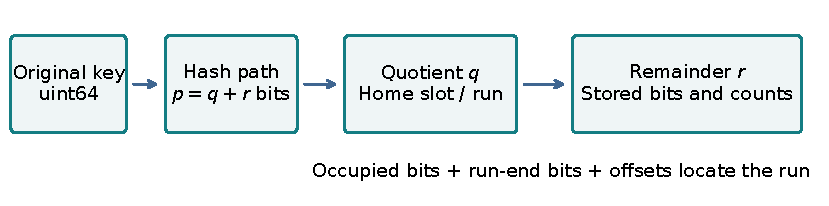
\includegraphics[width=0.94\linewidth]{cqf_layout.pdf}
\caption{Conceptual CQF path. Hashing, table geometry and counting are separate choices. The diagram illustrates the representation; it is not a memory dump of a measured run.}
\label{fig:cqf-layout}
\end{figure}

\subsection{Three end-to-end paths}
\begin{table}[!htbp]\centering\small
\caption{Hash paths evaluated with $p=q+r$ fingerprint bits. The external mixer is recomputed inside every timed insert, query and deletion loop.}
\label{tab:hash-paths}
\begin{tabular}{L{2.25cm}L{6.4cm}L{4.1cm}}\toprule
\textbf{Driver mode}&\textbf{Mapping before CQF run access}&\textbf{Cost included}\\\midrule
\texttt{default}&$\mathrm{MurmurHash64A}(x,\mathrm{seed}=0)\bmod 2^p$&Internal key hashing and CQF operation\\
\texttt{invertible}&Reference Thomas Wang integer mixer restricted to $p$ bits&Internal integer mixing and CQF operation\\
\texttt{none}&$\mathrm{SplitMix64}(x)\;\&\;(2^p-1)$, then \texttt{QF\_HASH\_NONE}&External mixing and CQF operation\\\bottomrule
\end{tabular}
\end{table}


Each path uses the same mapping for insertion, successful queries, negative queries and deletion. Precomputing this external hash outside the timed loop would remove work paid by the other modes. We explicitly include it. Therefore \texttt{none} means that the CQF performs no additional internal hash, not that the experiment has no hashing cost.

\subsection{What invertibility does and does not mean}
The reference invertible mixer is a permutation of the configured $p$-bit domain. That property does not preserve all original keys here: our integer inputs span a wider domain than $p=29$ in the 996k control or $p=36$ at 67M. The path projects keys into a smaller domain, where different original keys can collide. It must not be described as collision-free or as giving zero FPR. The external SplitMix64 path also loses information when masked to $p$ bits, despite using a full-width mixer first.

The default CQF path reduces modulo a runtime range stored as a 128-bit integer, whereas our external path uses a direct mask for its power-of-two domain. Thus range reduction and API-path work are part of the comparison, not just the mixer arithmetic. Both geometry and hash path affect the addresses touched by CQF operations. Consequently, a change in end-to-end throughput can reflect instruction cost, changed fingerprint collisions and changed run access, rather than pure hash-function latency. We make no standalone hash-cycle claim and no cryptographic or adversarial-input claim.

\subsection{Controlled experiment matrix}
Further source-level details for both internal mappings are given in Appendix~\ref{app:hash-details}. We run all three modes on both distributions with three timing repetitions and 10M negatives. The 996,148-operation control uses $q=20,r=9$ and includes occurrence-by-occurrence deletion. The 67M study uses $q=27,r=9$ and measures insertion and both query classes; deletion is omitted there by design. Large-scale deletion is still measured in the seven-filter comparison. Memory is identical across modes at a fixed scale. This isolates the hash-path choice within that configuration, while the change of $q$ prevents treating the two scales as one pure hash microbenchmark.
\clearpage

\section{Seven-Filter Results at 67M Uniform Operations}
\label{sec:uniform}
Every filter completes the uniform workload. Table~\ref{tab:uniform-large} compares supported online operations and query rates, while the immutable filters' construction costs are examined separately in Section~\ref{sec:static}. The table gives throughput means and sample standard deviations over three repetitions. A dash means the operation is unsupported; it is not a zero measurement.

\begin{table}[!htbp]\centering\small
\caption{New 67M uniform results at nominal target $1/512$. Rates are millions of operations or queries per second, mean $\pm$ sample SD. Memory is final footprint in decimal MB; Counting Bloom includes an estimated overflow-map allowance.}
\label{tab:uniform-large}
\begin{tabular}{@{}lrrrrr@{}}
\toprule
\textbf{Filter} & \textbf{Insert} & \textbf{Positive} & \textbf{Negative} & \textbf{Delete} & \textbf{MB} \\
\midrule
CQF & 1.47 $\pm$ 0.05 & 9.23 $\pm$ 0.48 & 12.80 $\pm$ 1.59 & 1.45 $\pm$ 0.03 & 186.808 \\
Cuckoo & 21.43 $\pm$ 1.25 & 25.14 $\pm$ 1.15 & 23.93 $\pm$ 5.70 & 23.46 $\pm$ 2.33 & 201.327 \\
Bloom & 11.88 $\pm$ 1.02 & 16.20 $\pm$ 1.09 & 19.25 $\pm$ 0.92 & \na & 108.743 \\
Counting Bloom & 6.43 $\pm$ 0.40 & 7.96 $\pm$ 0.71 & 12.99 $\pm$ 0.18 & 3.96 $\pm$ 0.32 & 434.973 \\
Blocked Bloom & 12.56 $\pm$ 1.28 & 12.22 $\pm$ 1.05 & 23.83 $\pm$ 1.95 & \na & 130.492 \\
XOR & \na & 18.34 $\pm$ 0.23 & 16.87 $\pm$ 2.24 & \na & 92.711 \\
Fuse-style & \na & 15.11 $\pm$ 2.84 & 17.44 $\pm$ 0.19 & \na & 94.372 \\
\bottomrule
\end{tabular}

\end{table}

\begin{figure}[!htbp]\centering
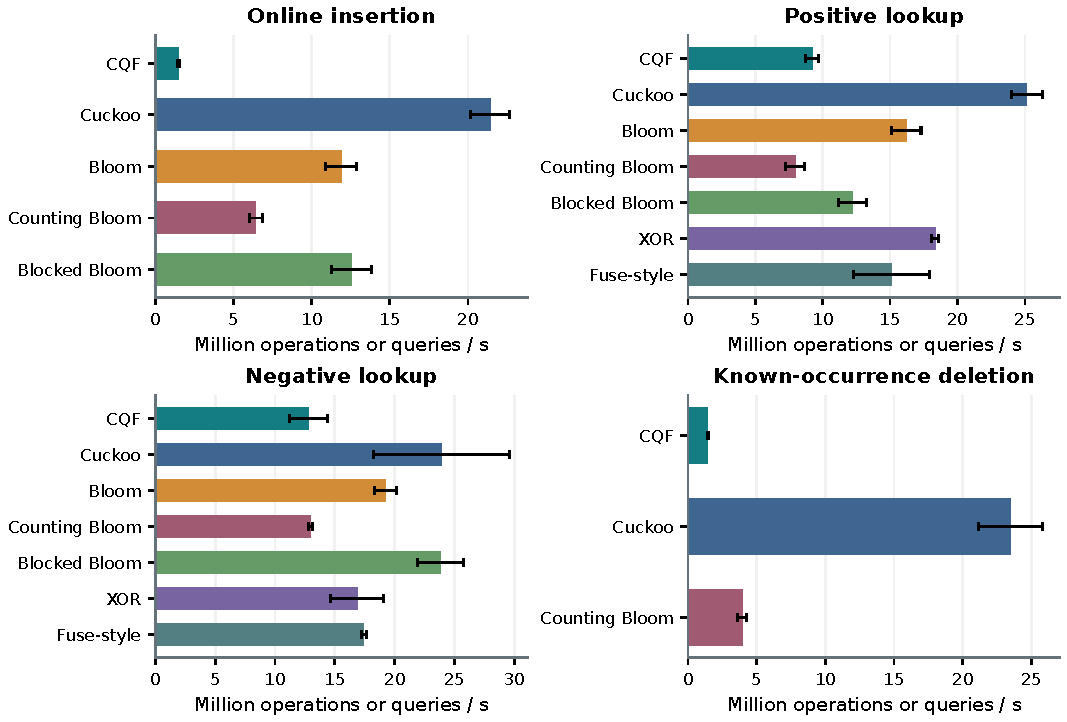
\includegraphics[width=\linewidth]{uniform_operations.pdf}
\caption{Supported operations on the 67M uniform stream. Bars show mean throughput and whiskers show one sample SD across three runs. Static filters appear in query panels only. The relative ranking is specific to these implementations and this translated execution environment.}
\label{fig:uniform}
\end{figure}

At this scale, \UniformFastestQuery{} reaches \UniformFastestQueryRate{}\,million successful queries per second. CQF achieves \CqfPositiveUniformLarge{}\Mops{} for the same query class and \CqfNegativeUniformLarge{}\Mops{} for negative queries. These results do not establish a universal advantage for one AMQ family: counting, deletion and immutable construction impose different costs, and the implementations use different hash and access paths.

The primary CQF occupies \PrimaryCqfMemory{}\,MB at about 50\% distinct load. It is therefore larger than the \BloomMemoryLarge{}\,MB Bloom filter, reversing the earlier report's three-filter space ordering. Equation~\ref{eq:cqf-sizing} explains the reversal: the allocation doubles when the workload crosses a power-of-two capacity boundary. CQF's occupied-slot count after insertion is \UniformOccupiedLarge{}, whereas its number of stored fingerprints is \UniformStoredLarge{}; colliding keys can share a fingerprint counter.
\finding{The large-scale comparison changes the space story as well as the speed story. A near-full CQF and a half-full CQF are different operating points.}
\clearpage

\section{Repeated Keys: Completion, Counters and Space}
\label{sec:skew}
The skewed stream contains 67M operations but only \NumDistinctLarge{} distinct keys. Its most frequent key occurs \MaxFrequencyLarge{} times. This distinction changes the task: a set-membership filter can represent each distinct member once, while a counting filter must also preserve the multiplicities through deletion.

\begin{table}[!htbp]\centering\small
\caption{New 67M skewed results at nominal target $1/512$. Rates are means $\pm$ sample SD in M/s. Static filters represent $D$ members and answer the original $N$ positive queries. ``Failed'' refers to incomplete construction; the accepted Cuckoo prefix is reported separately.}
\label{tab:zipf-large}
\begin{tabular}{@{}lrrrrr@{}}
\toprule
\textbf{Filter} & \textbf{Insert} & \textbf{Positive} & \textbf{Negative} & \textbf{Delete} & \textbf{MB} \\
\midrule
CQF & 4.31 $\pm$ 0.05 & 29.06 $\pm$ 2.17 & 18.21 $\pm$ 3.78 & 2.30 $\pm$ 0.15 & 186.808 \\
Cuckoo & Failed & Failed & Failed & Failed & 201.327 \\
Bloom & 74.58 $\pm$ 26.11 & 72.34 $\pm$ 12.43 & 44.39 $\pm$ 3.89 & \na & 0.372 \\
Counting Bloom & 12.16 $\pm$ 0.67 & 15.24 $\pm$ 0.66 & 30.14 $\pm$ 6.68 & 11.65 $\pm$ 1.49 & 9.235 \\
Blocked Bloom & 65.93 $\pm$ 3.60 & 48.77 $\pm$ 2.13 & 50.41 $\pm$ 3.56 & \na & 0.446 \\
XOR & \na & 101.84 $\pm$ 6.19 & 89.80 $\pm$ 2.03 & \na & 0.317 \\
Fuse-style & \na & 102.12 $\pm$ 5.15 & 85.95 $\pm$ 10.35 & \na & 0.333 \\
\bottomrule
\end{tabular}

\end{table}

Cuckoo accepts 24 of 67M insertion operations, a fraction of roughly $3.6\times10^{-7}$. The fixed stream quickly repeats the same key more often than the bucket pair can accommodate. We retain this outcome as a capability result and suppress its partial-run speed and FPR. It does not imply that deduplicating before a set-only Cuckoo build would fail; that would be a different experiment and would not preserve repeated-copy counts.

CQF and Counting Bloom both complete the full stream and all one-occurrence deletions. Bloom and Blocked Bloom also consume every insertion, but offer set membership without deletion. CQF's skewed insertion rate is \CqfInsertSkewLarge{}\Mops{}, compared with \CqfInsertUniformLarge{}\Mops{} on uniform data. Concentrated accesses and counter reuse are consistent with the improvement; we have not measured cache misses or isolated their individual effects.

\begin{figure}[!htbp]\centering
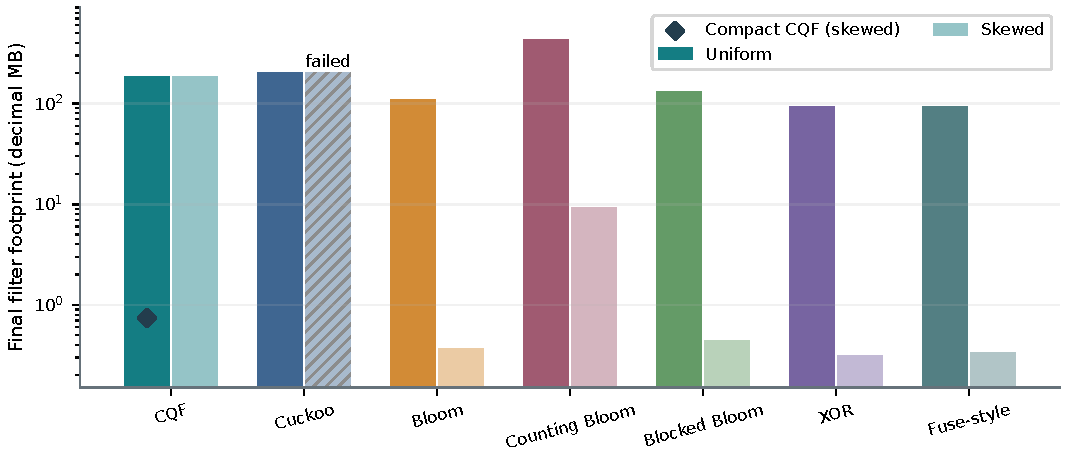
\includegraphics[width=\linewidth]{skew_space.pdf}
\caption{Final footprints under uniform and skewed input at 67M operations. The logarithmic scale keeps small distinct-set structures visible. Cuckoo's failed skewed allocation is marked explicitly. The extra CQF point is a separately sized, one-run sensitivity result; its FPR differs from the primary CQF.}
\label{fig:skew-space}
\end{figure}

The primary CQF reserves \PrimaryCqfMemory{}\,MB from $N$ even though only \SkewOccupiedLarge{} slots are occupied after insertion. By contrast, the Bloom family and immutable filters are allocated from $D$. We therefore also test a separate $2^{19}$-slot CQF at $r=9$ on the same complete skewed stream. It accepts and deletes all 67M occurrences using \CompactMemory{}\,MB. Its measured FPR is \CompactFpr{}, against the $D/2^{28}$ estimate of \CompactExpectedFpr{}. This is a valid target-satisfying operating point in this sample, with less spare capacity and a higher FPR than the primary CQF. Counting Bloom's reported footprint is \CompactCbfMemoryRatio{} times that of this compact CQF, with different achieved accuracy and update rates. This sensitivity point is not a general automatic-sizing algorithm or a proof of minimum capacity.
\finding{Counter compression and allocation policy are separate. A fixed operation-sized CQF can hide the space benefit of counting; a documented capacity sensitivity exposes it without changing the primary comparison.}
\clearpage

\section{Immutable Construction and Accuracy}
\subsection{The cost of building a static filter}
\label{sec:static}
A static filter can be small and fast to query because it receives the complete set before construction. That advantage comes with a cost: adding a new member generally requires rebuilding. Table~\ref{tab:static} includes preparation so that this work does not disappear from the comparison.

\begin{table}[!htbp]\centering\small
\caption{Static construction at 67M input operations. Times are mean seconds over three repetitions; rate columns are means of per-repeat rates in millions per second. Build-only rate uses $D$; end-to-end rate uses $N$ and includes preparation. The latter is stream-processing throughput, not an online insert rate.}
\label{tab:static}
\begin{tabular}{@{}llrrrr@{}}
\toprule
\textbf{Input} & \textbf{Filter} & \textbf{Prep (s)} & \textbf{Build (s)} & \textbf{Build (M keys/s)} & \textbf{Total (M ops/s)} \\
\midrule
Uniform & XOR & 0.447 & 16.640 & 4.09 & 3.99 \\
Uniform & Fuse-style & 0.447 & 10.878 & 6.44 & 6.20 \\
Zipfian & XOR & 2.139 & 0.012 & 18.98 & 31.41 \\
Zipfian & Fuse-style & 2.139 & 0.011 & 20.57 & 31.42 \\
\bottomrule
\end{tabular}

\end{table}

\begin{figure}[!htbp]\centering
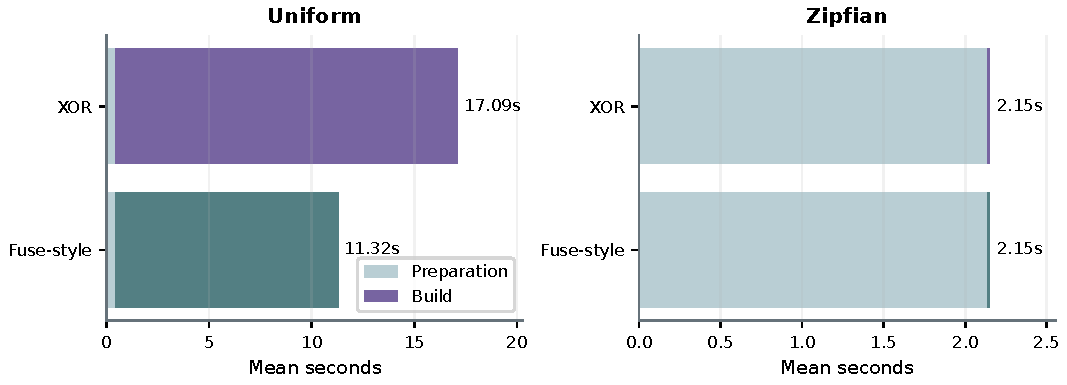
\includegraphics[width=0.96\linewidth]{static_preparation.pdf}
\caption{Mean preparation and build time for the immutable filters. Both are charged the shared preparation step as if built independently from the raw stream. In the actual driver the distinct-key preparation is computed once and reused.}
\label{fig:static-cost}
\end{figure}

For uniform input, preparation is a copy because the audit has verified that the stream is distinct. For skewed input, it sorts and deduplicates all 67M values before the much smaller set is built. Consequently, a high build-only rate on $D$ should not be confused with the end-to-end cost of processing $N$ input operations. Positive lookup rates also benefit from the frequency-weighted query stream, whose hottest keys are revisited often.

XOR uses 9-bit fingerprints at the primary target. The Fuse-style variant uses 10 bits. Its extra bit approximately halves the nominal FPR but also increases storage; it can therefore be larger than XOR here despite the Fuse family's more compact graph layout. We are comparing the actual configured implementations, rather than claiming an equal-accuracy contest between their theoretical storage bounds. Their final packed arrays do not include the substantial graph workspaces required during construction.

\subsection{Why preprocessing changes the construction story}
For skewed input, XOR's build stage takes only about 0.012 seconds, but preparation takes about 2.139 seconds. More than 99\% of the combined time is therefore spent producing the distinct set. The two immutable filters finish in almost the same end-to-end time on this stream even though their build-only rates differ. Under uniform input, the graph build dominates instead: total preparation-plus-build time is about 17.09 seconds for XOR and 11.32 seconds for the Fuse-style variant. The bottleneck changes with the data, not only with the filter family.

\subsection{A lifetime view of an immutable snapshot}
Construction is paid again when a snapshot is rebuilt. If a filter requires preparation time $P$, build time $B$, and then serves $L$ queries at average filter cost $c$, the corresponding filter-only lifetime cost is $P+B+Lc$. This accounting separates a frequently rebuilt snapshot from a long-lived one without treating batch construction as an online insertion rate. Our measurements supply $P$, $B$ and query batch costs; the application must supply its rebuild frequency and query volume. They do not yet supply peak construction memory or the cost of replacing a live snapshot.
\finding{Deduplication makes the stored set small, but the original stream still has to be processed. A static filter should be compared using preparation, construction and the expected lifetime of the snapshot.}
\clearpage

\subsection{Accuracy is a measured rate with uncertainty}
At 67M uniform operations, the half-full primary CQF is expected to have FPR near $0.499\times2^{-9}\approx0.000975$, not exactly the nominal $1/512\approx0.001953$. Under skew, the operation-sized CQF has many fewer distinct fingerprints and a much smaller expected collision rate. Ordinary Bloom and Counting Bloom remain near their nominal target; guarded Blocked Bloom measures about $0.000974$, roughly half that target. These are different achieved operating points.

\begin{figure}[!htbp]\centering
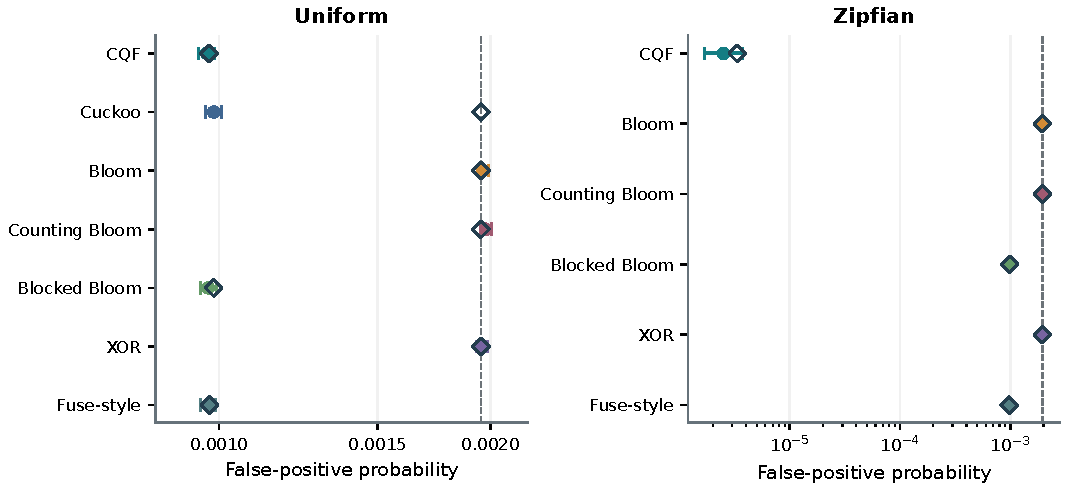
\includegraphics[width=\linewidth]{accuracy_intervals.pdf}
\caption{First-run measured FPR with 95\% Wilson intervals, using 10M negatives for each distribution. Diamonds indicate structure-specific estimates (the full-bucket reference value for Cuckoo); the dashed line marks the common nominal target. Cuckoo's failed skewed case is omitted. Cuckoo has a different random hash realization in each repetition; its repeat range is preserved in the accompanying table.}
\label{fig:accuracy}
\end{figure}

\begin{table}[!htbp]\centering\small
\caption{67M accuracy detail. Intervals use the first repetition and $Q=10$M, without pooling repeated copies of the same queries. The last column gives the range across the three raw timing repetitions. FPRs and interval endpoints are in units of $10^{-3}$.}
\label{tab:accuracy}
\begin{tabular}{@{}llrrr@{}}
\toprule
\textbf{Input} & \textbf{Filter} & \textbf{First FPR} & \textbf{95\% interval} & \textbf{Repeat range} \\
\midrule
Uniform & CQF & 0.9692 & [0.9501, 0.9887] & 0.9692 \\
Uniform & Cuckoo & 0.9865 & [0.9672, 1.0062] & 0.9661--0.9865 \\
Uniform & Bloom & 1.9616 & [1.9344, 1.9892] & 1.9616 \\
Uniform & Counting Bloom & 1.9771 & [1.9498, 2.0048] & 1.9771 \\
Uniform & Blocked Bloom & 0.9730 & [0.9539, 0.9925] & 0.9730 \\
Uniform & XOR & 1.9597 & [1.9325, 1.9873] & 1.9597 \\
Uniform & Fuse-style & 0.9725 & [0.9534, 0.9920] & 0.9725 \\
Skewed & CQF & 0.0025 & [0.0017, 0.0037] & 0.0025 \\
Skewed & Bloom & 1.9577 & [1.9305, 1.9853] & 1.9577 \\
Skewed & Counting Bloom & 1.9276 & [1.9006, 1.9550] & 1.9276 \\
Skewed & Blocked Bloom & 0.9742 & [0.9551, 0.9937] & 0.9742 \\
Skewed & XOR & 1.9322 & [1.9052, 1.9596] & 1.9322 \\
Skewed & Fuse-style & 0.9810 & [0.9618, 1.0006] & 0.9810 \\
\bottomrule
\end{tabular}

\end{table}

For the fixed-hash structures, repeated runs reproduce the same false-positive outcomes. Cuckoo's range also reflects its fresh random hash coefficients. A rate slightly above the nominal target can arise from finite sampling and from the approximation used for sizing; the confidence interval and implementation model provide the relevant context. A wider multi-seed experiment would be needed to establish a robust accuracy guarantee or to compare very small differences between mixers.
\finding{A lower observed FPR can result from spare capacity, a guard bit or fewer distinct members. It should be interpreted together with the memory and sizing policy that produced it.}
\clearpage

\section{Hash-Mode Results}
\label{sec:hash-results}
The controlled study keeps CQF memory identical across modes: 1,472,416 bytes in the 996,148-operation control and 186,807,707 bytes at 67M. Figure~\ref{fig:hash-speedup} expresses each mean rate relative to the default path at the same scale and distribution. Ratios compare means; the accompanying raw tables retain the three individual runs.

\begin{figure}[!htbp]\centering
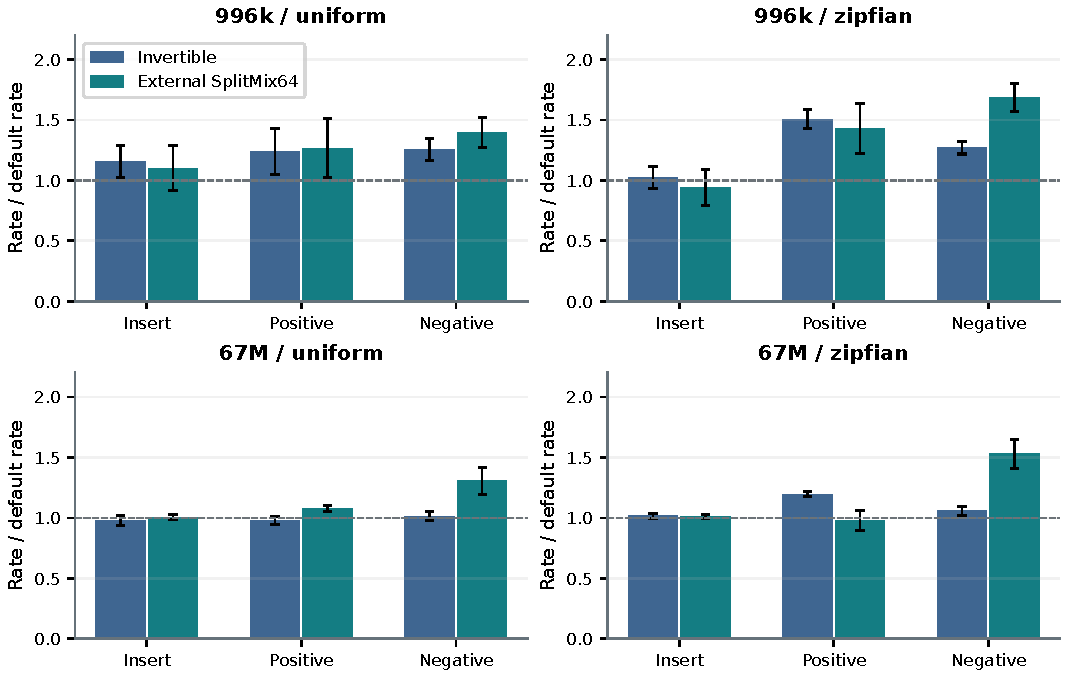
\includegraphics[width=\linewidth]{hash_speedups.pdf}
\caption{End-to-end CQF rate relative to default MurmurHash ($1\times$). The 996k control uses $q=20$; the 67M study uses $q=27$. Insertions and both query classes include the corresponding hash cost. Error bars show an approximate propagated descriptive SD, assuming independent run noise; they are not confidence intervals for the ratios.}
\label{fig:hash-speedup}
\end{figure}

At 67M uniform input, external SplitMix64 changes the negative-query rate from \HashDefaultNegativeUniform{} to \HashExternalNegativeUniform{}\Mops{}, a ratio of \HashExternalNegativeUniformRatio{}$\times$. Its uniform insertion ratio is \HashExternalInsertUniformRatio{}$\times$. On skewed input, its negative-query ratio is \HashExternalNegativeSkewRatio{}$\times$, while its insertion ratio is \HashExternalInsertSkewRatio{}$\times$. These differences show why we do not describe one mode as an unconditional improvement for every operation.

\begin{table}[!htbp]\centering\small
\caption{67M hash-path accuracy, first repetition with 10M negatives. The estimate uses the distinct original-key count over the configured fingerprint domain. Invertible mode retains a non-zero collision probability for these wider input keys.}
\label{tab:hash-accuracy}
\begin{tabular}{@{}llrrr@{}}
\toprule
\textbf{Input} & \textbf{Path} & \textbf{Measured} & \textbf{95\% interval} & \textbf{Estimate} \\
\midrule
Uniform & Default & $9.69\times10^{-4}$ & [$9.50\times10^{-4}$, $9.89\times10^{-4}$] & $9.75\times10^{-4}$ \\
Uniform & Invertible & $9.66\times10^{-4}$ & [$9.47\times10^{-4}$, $9.86\times10^{-4}$] & $9.75\times10^{-4}$ \\
Uniform & External & $9.79\times10^{-4}$ & [$9.60\times10^{-4}$, $9.98\times10^{-4}$] & $9.75\times10^{-4}$ \\
Zipfian & Default & $2.50\times10^{-6}$ & [$1.69\times10^{-6}$, $3.69\times10^{-6}$] & $3.33\times10^{-6}$ \\
Zipfian & Invertible & $3.70\times10^{-6}$ & [$2.68\times10^{-6}$, $5.10\times10^{-6}$] & $3.33\times10^{-6}$ \\
Zipfian & External & $3.50\times10^{-6}$ & [$2.52\times10^{-6}$, $4.87\times10^{-6}$] & $3.33\times10^{-6}$ \\
\bottomrule
\end{tabular}

\end{table}

The hash choices do not change the CQF's counter representation or memory allocation. Their FPR estimates are consequently the same within a workload, while the measured samples differ with the mapping. At the skewed 67M operating point, the expected number of false positives is only about 33 in 10M queries, so rate ratios can look large even when the absolute difference is a few queries. Neither the lowest observed rate nor the fastest one-operation result is enough to nominate a universally best mixer.

The most defensible practical outcome is to expose the hash choice, measure the operation mix that matters, and verify positive recognition and accuracy after changing it. We retain the default path for the primary seven-filter comparison to avoid mixing a hash substitution with the filter-family comparison.
\clearpage

\section{Scale, Geometry and the Earlier Results}
\subsection{What changes from 1M to 67M}
Figure~\ref{fig:scaling} compares the new small and large experiments run in the same environment. It holds the nominal target and implementation family fixed, but does not hold every table load fixed. CQF moves from 47.68\% to 49.92\% distinct uniform load; Cuckoo's capacity rounding changes its load more substantially. The stream length, memory footprint and allocation geometry all change together. The plot therefore measures scale under the implemented sizing policies, not cache capacity in isolation.

\begin{figure}[!htbp]\centering
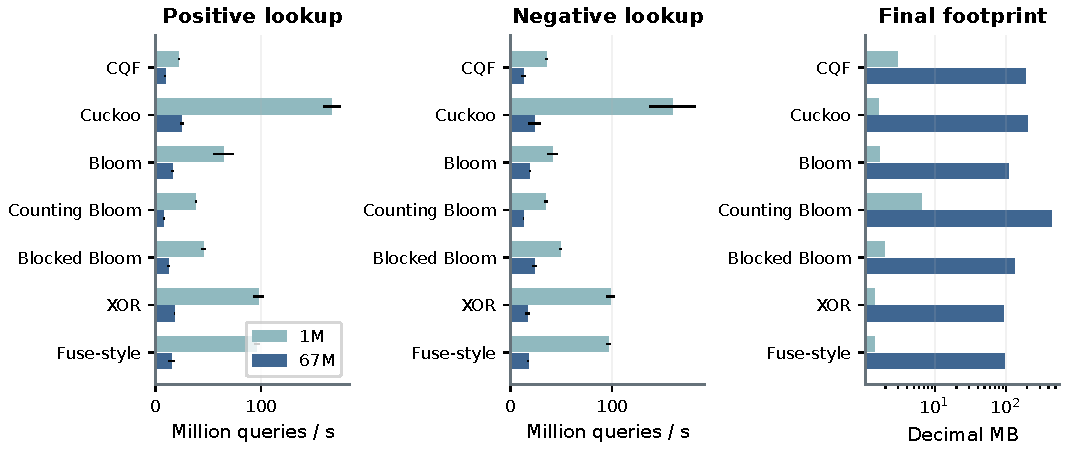
\includegraphics[width=\linewidth]{scale_comparison.pdf}
\caption{New 1M and 67M uniform query throughput and final footprint at nominal target $1/512$. Whiskers show one sample SD for throughput. Memory and capacity changes accompany the larger stream.}
\label{fig:scaling}
\end{figure}

The earlier report suggested that small filters fitting in cache could explain part of its speed ordering. The new data make that explanation more testable, but do not prove it: there are no hardware-counter measurements, controlled cache-flush experiments or native x86 runs here. Rosetta translation and fixed execution order add further reasons to keep the conclusion descriptive. The supported conclusion is that the ranking and operation costs depend on scale and configuration in this harness.

\subsection{Matched-operation-count CQF geometry sensitivity}
To separate the requested operation count from the allocation boundary, we replay 63,753,420 uniform operations against both $2^{26}$ and $2^{27}$ CQF slots, with $r=9$ and the default hash. Both configurations complete the full insert and positive-query workload in each of three repetitions. Deletion is omitted in this supplementary timing study.

\begin{table}[!htbp]\centering\small
\caption{Matched-$N$ CQF sensitivity. Rates are means $\pm$ sample SD in M/s. Holding $r=9$ while changing $q$ also changes the fingerprint width and collision estimate.}
\label{tab:geometry-control}
\begin{tabular}{@{}lrrrrr@{}}
\toprule
\textbf{Slots} & \textbf{MB} & \textbf{First FPR} & \textbf{Insert} & \textbf{Positive} & \textbf{Negative} \\
\midrule
$2^{26}$ & 93.437 & $1.85\times10^{-3}$ & 1.51 $\pm$ 0.01 & 7.63 $\pm$ 0.04 & 10.45 $\pm$ 0.07 \\
$2^{27}$ & 186.808 & $9.26\times10^{-4}$ & 1.58 $\pm$ 0.00 & 9.84 $\pm$ 0.07 & 14.25 $\pm$ 0.51 \\
\bottomrule
\end{tabular}

\end{table}

The larger table doubles final memory and reduces distinct load from 95\% to 47.5\%. It also increases $p=q+r$ from 35 to 36 bits, approximately halving the expected FPR. Any speed difference is a combined geometry effect involving run lengths, address range and fingerprint collisions. The near-full table uses \GeometrySmallBits{} bits per uniform key, close to the reference paper's 11.71; the doubled table uses \GeometryLargeBits{}. This control separates the requested operation count from the allocation boundary, while retaining the stated fingerprint-width confound.

An application must also account for the work caused by false positives. If an absent-key lookup costs $c_{\mathrm{filter}}$ in the filter and a positive answer triggers an additional cost $C$, its expected cost is $c_{\mathrm{filter}}+\hat p C$ under that lookup model. A more accurate filter can therefore be worthwhile even when its own query is slower. We do not assign a measured value to $C$ here; it is a property of the application that the microbenchmark cannot determine.
\clearpage

\subsection{Comparison with the mid-semester report and reference paper}
\begin{table}[!htbp]\centering\small
\caption{Uniform reference context for the original three filters. Insert/positive/negative rates are in M/s. Literature values are from Table~1(a) of Pandey et al.; earlier values are transcribed from the supplied report. Archived 67M values are preserved from the input ZIP; new values are measured in this session. These are separate environments, configurations and protocols, not speedup trials.}
\label{tab:history}
\begin{tabular}{@{}llrrr@{}}
\toprule
\textbf{Result source} & \textbf{Filter} & \textbf{Insert} & \textbf{Positive} & \textbf{Negative} \\
\midrule
Reference paper & CQF & 11.19 & 11.16 & 25.93 \\
Reference paper & Cuckoo & 14.25 & 18.87 & 18.84 \\
Reference paper & Bloom & 2.84 & 2.55 & 11.56 \\
Mid-semester & CQF & 8.33 & 17.06 & 23.91 \\
Mid-semester & Cuckoo & 22.75 & 125.47 & 128.23 \\
Mid-semester & Bloom & 30.22 & 30.16 & 31.04 \\
Archived 67M & CQF & 3.85 & 7.03 & 9.92 \\
Archived 67M & Cuckoo & 18.15 & 19.22 & 18.76 \\
Archived 67M & Bloom & 6.61 & 7.44 & 12.30 \\
New 67M & CQF & 1.47 & 9.23 & 12.80 \\
New 67M & Cuckoo & 21.43 & 25.14 & 23.93 \\
New 67M & Bloom & 11.88 & 16.20 & 19.25 \\
\bottomrule
\end{tabular}

\end{table}

The mid-semester baseline used 996,148 operations and a CQF near 95\% load. Its values are retained exactly as reported, even where the supplied archive also contains later validation numbers. The supplied archive's 67M study extends the original three filters and supplies an earlier hash study; it does not contain an all-seven 67M measurement. Our new large experiment supplies that missing comparison.

The reference paper uses an Intel Skylake machine and samples performance through successive load levels. It excludes input generation, as we do, but its implementation versions and hardware differ. Its skewed-data result also identifies the ordinary Cuckoo filter's duplicate limitation, while our exact stopping point is determined by our stream. The meaningful agreements are completion behaviour and the roles of counting, space and load; the absolute rates are contextual reference values~\cite{pandey2017}.

The paper's CQF-over-Counting-Bloom speed ordering is not reproduced uniformly in our new results. Our Counting Bloom reaches \CountingBloomInsertSkewLarge{}\Mops{} on skewed insertion, compared with \CqfInsertSkewLarge{}\Mops{} for CQF. CQF leads in positive-query throughput, while Counting Bloom leads in negative-query throughput. The packed-counter overflow implementation, distinct-aware sizing and translated host all differ from the published setup. These measurements describe the configured implementations in this study and leave native, matched-configuration replication as follow-up work.

The public repository ends at commit \texttt{fe184baa6933} (9 November 2026), which adds hash and paper-scale studies~\cite{projectcode}. The supplied Phase-3 ZIP adds the four new filters and is our experimental source snapshot. The public API returned no pull-request entries; this provenance is a verified source history, not a PR timeline.

\subsection{What can be carried across these comparisons}
Three kinds of agreement should be distinguished. \textit{Semantic agreement} asks whether the implementation performs the required task: CQF and Counting Bloom retain repeated occurrences, while this Cuckoo configuration runs out of room for copies. \textit{Configuration agreement} asks whether the same capacity, fingerprint width and cardinality knowledge were used. \textit{Numerical agreement} asks whether rates match after hardware, software and timing conventions are controlled. This study establishes the first, records the second, and gives contextual rather than replicated evidence for the third.

The distinction matters even at small scale. Moving from 996,148 to exactly 1M operations adds only about 0.39\% more input, yet crosses the CQF allocation boundary and doubles its slot count. The archived and new 67M Zipf generators also realize slightly different distinct sets: 229,118 versus 229,115 keys. The difference is small, but it illustrates why the report keeps separate input audits instead of treating a shared seed as proof of identical data. Our extension adds a common seven-family record and controls that make these operating points visible; it does not convert cross-environment rates into algorithmic speedups.
\clearpage

\subsection{Sensitivity to the nominal error target}
We also replay the 67M streams at nominal targets $1/256$ and $1/1024$. These two supplementary configurations have one timing pass each; only the main $1/512$ configuration has three. The sweep checks parameterization and space/accuracy trends. It does not provide repeated performance evidence at every error target.

\begin{figure}[!htbp]\centering
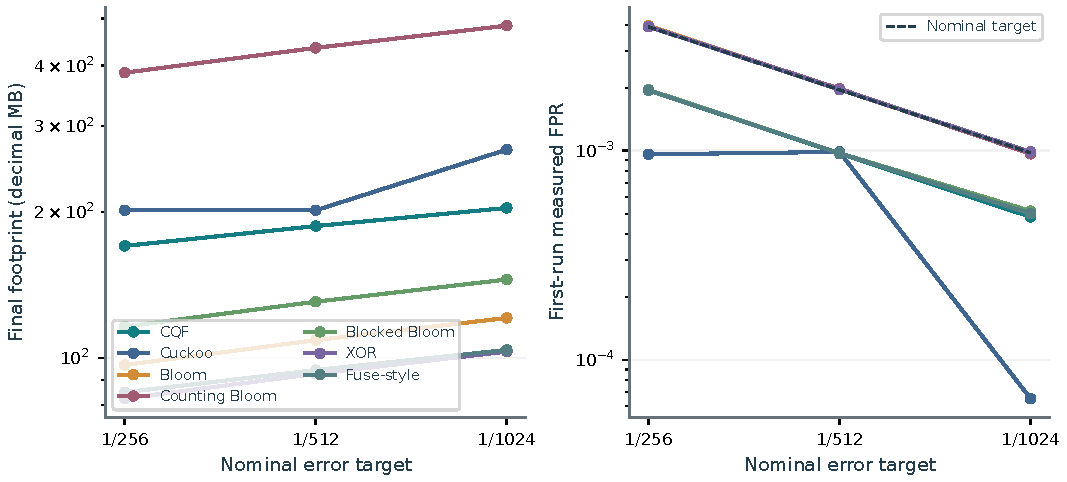
\includegraphics[width=\linewidth]{fpr_sensitivity.pdf}
\caption{67M uniform space and measured FPR across three nominal targets. Each point uses the first pass; the end targets are single-pass supplementary experiments. Fuse-style retains one guard bit beyond XOR. Changes in achieved accuracy and footprint should be read together.}
\label{fig:sensitivity}
\end{figure}

\begin{table}[!htbp]\centering\small
\caption{Uniform target sweep at 67M operations. Column labels 256, 512 and 1024 denote nominal targets $1/256$, $1/512$ and $1/1024$. Memory is decimal MB; first-pass FPRs are in units of $10^{-3}$. The end targets have one timing pass, so this table describes space and sampled accuracy, not repeated speed rankings.}
\label{tab:target-sweep}
\begin{tabular}{@{}lrrrrrr@{}}
\toprule
\textbf{Filter} & \textbf{MB: 256} & \textbf{MB: 512} & \textbf{MB: 1024} & \textbf{FPR: 256} & \textbf{FPR: 512} & \textbf{FPR: 1024} \\
\midrule
CQF & 170.02 & 186.81 & 203.60 & 1.9408 & 0.9692 & 0.4827 \\
Cuckoo & 201.33 & 201.33 & 268.44 & 0.9607 & 0.9865 & 0.0653 \\
Bloom & 96.66 & 108.74 & 120.83 & 3.9591 & 1.9616 & 0.9826 \\
Counting Bloom & 386.64 & 434.97 & 483.30 & 3.9207 & 1.9771 & 0.9662 \\
Blocked Bloom & 115.99 & 130.49 & 144.99 & 1.9535 & 0.9730 & 0.5149 \\
XOR & 82.41 & 92.71 & 103.01 & 3.9159 & 1.9597 & 0.9866 \\
Fuse-style & 84.93 & 94.37 & 103.81 & 1.9409 & 0.9725 & 0.5003 \\
\bottomrule
\end{tabular}

\end{table}

The CQF keeps $q=27$ throughout the sweep and increases $r$ from 8 to 10. Each additional remainder bit adds about 16.79\,MB to the primary allocation and approximately halves the collision estimate. Bloom-family storage also grows as the target tightens, with the number of probes rising from 8 to 10. Counting Bloom pays four bits per base cell before overflow, so the same sizing change carries a larger absolute space cost.

Cuckoo exposes a different parameter effect. Its supported fingerprint widths keep it at 12 bits for the first two targets, then move it to 16 bits for $1/1024$. Memory jumps from 201.33 to 268.44\,MB, while the measured FPR falls well below the requested target. A smooth nominal-target axis therefore need not produce a smooth space curve. The guard choices in Blocked Bloom and Fuse-style likewise leave them below the common target. Equalizing the target input is useful for checking the harness; comparing equal achieved accuracy would require selecting different configurations.
\finding{Accuracy is purchased in implementation-specific increments. The relevant comparison is the achieved error rate together with its storage and operation cost, not the target label alone.}
\clearpage

\section{Discussion, Limitations and Next Steps}
\subsection{Choosing a filter from the measured trade-offs}
The results support a capability-based choice. If a system only needs membership while constructing an immutable snapshot, XOR and the Fuse-style variant make compact final representations with three-cell queries. Their preparation, rebuild cost and construction workspace still have to fit the system. A continuously updated set needs a different comparison: Bloom and Blocked Bloom offer low-cost membership updates, while Cuckoo supports deletion when duplicate-copy pressure is manageable. A multiset that requires occurrence-by-occurrence deletion needs explicit counter behaviour.

\begin{table}[!htbp]\centering\small
\caption{How to use the evidence from this study. These are workload-specific considerations, not universal recommendations for every implementation of each family.}
\label{tab:selection}
\begin{tabular}{L{4.0cm}L{4.2cm}L{4.4cm}}\toprule
\textbf{Required behaviour}&\textbf{Candidates to examine}&\textbf{Cost that remains visible}\\\midrule
Membership with online additions&Bloom; Blocked Bloom&No supported deletion; different locality/space budgets\\
Known-member deletion with few repeats&Cuckoo; CQF; Counting Bloom&Capacity failures, counters and achieved FPR\\
Many repeated occurrences with deletion&CQF; Counting Bloom&Counter storage and conservative versus distinct-aware capacity\\
Immutable membership snapshot&XOR; Fuse-style&Preparation, build/rebuild work and unmeasured peak workspace\\
Changing CQF hash path&Default; invertible; external mixer&End-to-end operation mix and fingerprint-domain collisions\\\bottomrule
\end{tabular}
\end{table}

CQF's value in this study is the combination of compact fingerprint counting and deletion under repeated input, with a configurable hash path. Its primary operation-sized footprint also demonstrates how easily an allocation rule can hide that value. Counting Bloom provides a useful counter baseline, but overflow storage and per-probe updates change its cost under skew. Neither a fast membership query nor a small final array alone captures these differences.

\subsection{Reading separate query rates as an operation mix}
A workload rarely consists entirely of successful or unsuccessful queries. To make the two measured query classes easier to interpret, let $\alpha$ be the fraction of positive queries, and let $\bar c_+$ and $\bar c_-$ be their mean batch-derived costs in seconds per query. A simple sequential query-only model gives
\begin{equation}
R(\alpha)=\frac{1}{\alpha\bar c_+ +(1-\alpha)\bar c_-}.
\label{eq:query-mix}
\end{equation}
This is a calculation from the existing batches, not a newly timed mixed workload. It assumes that each class retains its measured average cost and excludes updates, construction and the underlying database lookup.

\begin{table}[!htbp]\centering\small
\caption{Calculated query-only throughput in M/s from mean per-query batch costs at 67M operations. The percentage gives $\alpha$, the fraction of positives. The skewed model preserves the measured frequency-weighted positive stream and uniform absent-key negatives. Cuckoo's incomplete skewed workload is unavailable.}
\label{tab:query-mix}
\begin{tabular}{@{}lrrr@{}}
\toprule
\textbf{Filter} & \textbf{Uniform: 50\% +} & \textbf{Uniform: 90\% +} & \textbf{Skewed: 50\% +} \\
\midrule
CQF & 10.67 & 9.47 & 21.91 \\
Cuckoo & 23.95 & 24.87 & \na \\
Bloom & 17.55 & 16.41 & 54.39 \\
Counting Bloom & 9.83 & 8.23 & 19.97 \\
Blocked Bloom & 16.08 & 12.78 & 49.46 \\
XOR & 17.46 & 18.16 & 95.32 \\
Fuse-style & 15.98 & 14.98 & 92.74 \\
\bottomrule
\end{tabular}

\end{table}

On uniform input, Cuckoo leads these query-only examples, but that result cannot satisfy a heavy-repeat counting requirement. In the skewed 50\% example, CQF reaches a calculated 21.91\,M/s against Counting Bloom's 19.97\,M/s: its faster positive queries offset its slower negatives at that particular mix. Changing the mix changes the balance. The immutable filters have high query-only rates on this skewed set, while their preparation and rebuild costs remain outside the model.

\clearpage

\subsection{Limits of the evidence}
\begin{itemize}
\item \textbf{Platform and repetitions.} These are single-threaded results from one translated x86-64 environment on Apple M2. We use three primary timing repetitions, one fixed input seed, a fixed operation order and no CPU affinity. Virtual CPU metadata is not a physical cache measurement. Timing SD describes this run set, not a cross-machine confidence interval.
\item \textbf{Capacity and cardinality knowledge.} Several filters use exact offline $D$, while primary CQF/Cuckoo allocations use $N$. The compact CQF study is a documented sensitivity point, not an online resizing policy. The geometry control changes both load and fingerprint width.
\item \textbf{Implementation scope.} The four added filters are scalar reference variants. Fuse-style is not the optimized Binary Fuse reference, and the Counting Bloom overflow design differs from the paper's baseline. We have not normalized every implementation to equal achieved FPR or equal memory.
\item \textbf{Accuracy and operation semantics.} Fixed-query repeats are not independent new accuracy samples. Cuckoo introduces fresh, unrecorded hash randomness. The tests exercise known inserted deletions; deleting arbitrary absent keys can damage other members in probabilistic deletion structures. We do not claim exact original-key counts after fingerprint collisions.
\item \textbf{System costs.} Final footprint excludes most process overhead and temporary construction storage. We do not evaluate SSD behaviour, concurrency, merging, adaptive queries, adversarial keys or benefits in a complete application.
\end{itemize}

\subsection{Validation behind the conclusions}
Validation spans four levels: supported operations, input labels, workload completion and result summaries (Table~\ref{tab:validation-levels}). A correct filter alone does not establish that an experiment is valid: contaminated negatives, partial workloads or misleading aggregation can still change the comparison. These checks connect the implementation to the reported evidence.

\begin{table}[!htbp]\centering\small
\caption{Checks supporting the reported comparisons. Timing variation is described separately by repeated measurements.}
\label{tab:validation-levels}
\begin{tabular}{L{2.0cm}L{5.3cm}L{5.3cm}}\toprule
\textbf{Level}&\textbf{Checked condition}&\textbf{Purpose}\\\midrule
Functional&Repeated-key decrements, overflow counters and positive recognition&Exercise supported membership/counting operations\\
Workload&Exact distinct count, maximum frequency, absent-key queries and file hashes&Establish the actual stream and its query labels\\
Run&Accepted, recognized and deleted counts; expected repetition counts&Separate complete tasks from capacity failures and partial runs\\
Summary&Unsupported-operation masking and raw-to-table regeneration&Keep dashes, failures, units and aggregates consistent\\\bottomrule
\end{tabular}
\end{table}

\subsection{Conclusion and focused future work}
We have extended the earlier three-filter baseline into a complete seven-family evaluation at 67M operations, added a controlled CQF hash-path study, and made the data and validation steps inspectable. The strongest conclusions are concrete: duplicate handling changes whether a workload completes; capacity rounding changes the space comparison; immutable filters require preparation and rebuild accounting; and hash-path gains depend on the operation and input distribution.

The next useful work follows directly from these findings. We would repeat the primary matrix on native x86-64 hardware with multiple input and filter seeds, compare configurations at matched achieved FPR and controlled memory budgets, and measure peak construction memory. For CQF specifically, we would test distinct-aware capacity rules with explicit counter headroom, then evaluate whether hash-path choices remain beneficial on application-generated keys. Lock-region tuning, heap-based merging and an application wrapper remain deferred directions from the earlier report; they are not presented as completed contributions here.

These steps have a natural order. Native runs and randomized repetition order would first test whether the main rate differences persist without translation and fixed-order effects. A matched-accuracy matrix would then show which space differences remain after spare capacity and guard bits are accounted for. Finally, application traces could supply the successful-query fraction, repetition pattern and false-positive penalty needed to evaluate the cost model above. This sequence would turn the present controlled comparison into stronger deployment evidence without treating unmeasured system behaviour as an explanation for the current numbers.

\finding{The main advance is a broader comparison that explains its own operating points. The measurements tell us when an implementation completes the task and what it pays for doing so.}
\FloatBarrier

\FloatBarrier
\clearpage
\section*{Data and Code Availability}
The accompanying artifacts provide the measurements and the steps used to turn them into this report. The code package contains the seven implementations, functional tests, experiment runners, raw repetitions, configuration records, workload audits and report-asset generator. The LaTeX package contains editable section files, vector figures, generated tables, the numeric macros used in the prose and a portable copy of the supporting CSVs. The supplied earlier progress report is retained for comparison, while the historical, archived and newly measured result sources remain explicitly distinguished.

The target-sweep table is generated from the first recorded pass at each target. The query-mix table is a separate analytical calculation from measured batch costs; its values are provided in \nolinkurl{data/query_mix_model.csv}. Neither addition represents a new timed experiment. This separation lets a reader check the calculations without confusing them with repeated performance evidence.

Large binary workloads and compiled executables are omitted from the ZIPs. Reproduction scripts regenerate the inputs, and saved manifests, cardinality audits and SHA-256 hashes allow the streams to be compared. The final source manifest identifies the packaged code; the separately named run-start manifest preserves the earlier snapshot. Exact timing and Cuckoo FPR values can vary on a rerun for the reasons described in the methodology. Appendix~\ref{app:repro} maps the files to experiments and gives the execution and regeneration commands.

\begingroup
\normalsize
\raggedright
\setlength{\bibsep}{7pt}
\setlength{\parskip}{0pt}
\bibliographystyle{unsrtnat}
\bibliography{references}
\endgroup
\clearpage
\appendix
\section{Reproducibility and Artifact Guide}
\label{app:repro}
The Overleaf package contains all figures, generated tables and the CSVs behind this report. The separate code package includes source, tests, archived outputs, the new raw measurements and the asset generator. Large binary workload files and compiled executables are omitted. Their manifest parameters, exact cardinality checks and SHA-256 hashes are retained under \texttt{results/report/} and copied into the LaTeX project's \texttt{reproducibility/} directory.

\begin{table}[!htbp]\centering\small
\caption{Evidence map for the report. Prefixes refer to files in \texttt{data/} in this LaTeX package and to the corresponding \texttt{results/} files in the code package.}
\begin{tabular}{L{4.0cm}L{8.7cm}}\toprule
\textbf{Experiment}&\textbf{Raw / configuration evidence}\\\midrule
Seven-filter 1M and 67M&\texttt{paper\_scale\_report\_*\_raw.csv}, \texttt{additional\_filters\_report\_*\_raw.csv}, combined \texttt{all\_filters\_report\_*} and configuration files\\
Hash modes&\texttt{hash\_modes\_report\_control\_raw.csv} and \texttt{hash\_modes\_report\_67m\_raw.csv}\\
Compact CQF and geometry&\texttt{compact\_zipf\_raw.csv}; \texttt{geometry\_control\_raw.csv}\\
Target sweep&Tags \texttt{report\_67m\_256} and \texttt{report\_67m\_1024}\\
Earlier report / archive&\texttt{archived\_bench.csv}; \texttt{archived\_paper\_scale\_1\_512.csv}\\
Audit and environment&\texttt{manifest\_*.txt}, \texttt{audit\_*.json}, \texttt{environment.txt}, \texttt{source\_manifest.json}, test/run logs\\\bottomrule
\end{tabular}
\end{table}

\textbf{Execution.} On Apple Silicon, create an \texttt{linux/amd64} Ubuntu 22.04 container and mount the extracted code folder at \texttt{/amq-benchmark}. Install the following dependencies inside the container, then run the experiment script from that folder:
\begin{lstlisting}[language=bash]
apt-get update
apt-get install -y build-essential libssl-dev python3 \
  python3-numpy python3-pandas python3-matplotlib time
cd /amq-benchmark
chmod +x scripts/*.sh
./scripts/run_report_experiments.sh
\end{lstlisting}
The script verifies functional tests, audits generated input files outside timing, runs the complete matrix, and validates supplementary completion before writing \texttt{COMPLETED.txt}. Changing library versions may change the realized Zipf stream, so compare audited hashes and cardinalities as well as the seed. Cuckoo's unrecorded per-process hash coefficients mean its exact FPR is not deterministically reproduced by the fixed workload alone.

\textbf{Plot and table generation.} From the code root, run the asset generator on the result files to regenerate vector figures, CSV summaries and numeric LaTeX macros. The supplied Overleaf ZIP already contains the generated assets; compiling it needs neither Python nor benchmark execution.
\begin{lstlisting}[language=bash]
python3 scripts/make_research_assets.py --out /path/to/latex-project
# In Overleaf: main.tex; pdfLaTeX; BibTeX handled automatically.
\end{lstlisting}

\textbf{Run integrity.} For complete dynamic rows, insertion and positive-recognition counts equal $N$. CQF and Counting Bloom deletion success counts equal $N$ in their full-delete experiments. Static rows recognize all $N$ positive queries after construction from $D$ distinct members. Cuckoo's incomplete skewed rows retain only the accepted count for comparison. The new workload audit and supplementary-run checks include regression tests for deliberate invalid inputs.

\textbf{Package scope.} The source ZIP is a local, audited extension of the supplied archive. No GitHub push or PR is implied. The restored upstream CQF and Cuckoo licenses remain in their source directories; local implementation and interpretation changes are recorded in \texttt{docs/REPORT\_AUDIT.md}.
\clearpage

\section{Complete Small-Scale and Hash Timing Tables}
\begin{table}[!htbp]\centering\small
\caption{New 1M-operation seven-filter results. Throughput means are in M/s; final footprint is in decimal MB. Dynamic insertions are measured over $N$ operations. Static build rates, shown in the build column only, use $D$ distinct keys and exclude preparation. Unsupported and incomplete-workload rates are dashes; the skewed Cuckoo row accepts only 24 operations. Full raw repetitions remain in the data files.}
\label{tab:small-full}
\begin{tabular}{@{}llrrrrrr@{}}
\toprule
\textbf{Input} & \textbf{Filter} & \textbf{Insert} & \textbf{Build} & \textbf{Positive} & \textbf{Negative} & \textbf{Delete} & \textbf{MB} \\
\midrule
Uniform & CQF & 1.86 & \na & 22.22 & 35.74 & 1.76 & 2.937 \\
Uniform & Cuckoo & 29.74 & \na & 167.23 & 159.38 & 47.36 & 1.573 \\
Uniform & Bloom & 78.64 & \na & 64.73 & 41.70 & \na & 1.623 \\
Uniform & Counting Bloom & 26.93 & \na & 38.20 & 34.74 & 20.37 & 6.492 \\
Uniform & Blocked Bloom & 60.66 & \na & 45.21 & 49.21 & \na & 1.948 \\
Uniform & XOR & \na & 17.98 & 97.99 & 98.50 & \na & 1.384 \\
Uniform & Fuse-style & \na & 21.24 & 96.22 & 96.34 & \na & 1.413 \\
Skewed & CQF & 4.40 & \na & 20.52 & 90.12 & 2.56 & 2.937 \\
Skewed & Cuckoo & \na & \na & \na & \na & \na & 1.573 \\
Skewed & Bloom & 101.00 & \na & 84.48 & 55.75 & \na & 0.023 \\
Skewed & Counting Bloom & 15.19 & \na & 17.95 & 42.93 & 13.04 & 0.556 \\
Skewed & Blocked Bloom & 70.80 & \na & 50.45 & 57.43 & \na & 0.028 \\
Skewed & XOR & \na & 16.25 & 117.85 & 115.87 & \na & 0.020 \\
Skewed & Fuse-style & \na & 15.56 & 112.45 & 110.16 & \na & 0.023 \\
\bottomrule
\end{tabular}

\end{table}

\begin{table}[!htbp]\centering\small
\caption{CQF hash study: mean throughput in M/s. The 996k control includes deletion; 67M deletion is omitted by design. Both use three timing repetitions and 10M negatives.}
\label{tab:hash-full}
\begin{tabular}{@{}lllrrrr@{}}
\toprule
\textbf{Scale} & \textbf{Input} & \textbf{Path} & \textbf{Insert} & \textbf{Positive} & \textbf{Negative} & \textbf{Delete} \\
\midrule
996k & Uniform & Default & 1.52 & 13.84 & 20.30 & 1.20 \\
996k & Uniform & Invertible & 1.75 & 17.12 & 25.47 & 1.43 \\
996k & Uniform & External & 1.67 & 17.53 & 28.35 & 1.47 \\
996k & Skewed & Default & 4.17 & 19.98 & 87.80 & 2.40 \\
996k & Skewed & Invertible & 4.28 & 30.08 & 111.55 & 2.45 \\
996k & Skewed & External & 3.93 & 28.57 & 148.03 & 2.42 \\
67M & Uniform & Default & 1.53 & 9.69 & 14.62 & \na \\
67M & Uniform & Invertible & 1.50 & 9.50 & 14.82 & \na \\
67M & Uniform & External & 1.54 & 10.42 & 19.10 & \na \\
67M & Skewed & Default & 4.38 & 30.56 & 20.72 & \na \\
67M & Skewed & Invertible & 4.46 & 36.59 & 21.92 & \na \\
67M & Skewed & External & 4.45 & 29.83 & 31.67 & \na \\
\bottomrule
\end{tabular}

\end{table}

\textbf{Aggregation convention.} The report recomputes mean rates from raw repetitions. Some legacy CSV-derived rates instead divide operation count by the mean duration; these two summaries need not be identical.

\textbf{Uncertainty convention.} In all plots, timing whiskers are descriptive sample SD unless stated otherwise. For $z=1.96$, the first-run Wilson FPR interval has centre and half-width
\[
 c=\frac{\hat p+z^2/(2Q)}{1+z^2/Q},\qquad
 w=\frac{z}{1+z^2/Q}\sqrt{\frac{\hat p(1-\hat p)}{Q}+\frac{z^2}{4Q^2}}.
\]
It describes random query sampling for the fixed filter realization and query distribution; it does not cover all input distributions or all possible hash seeds.
At tiny rates, a few positive answers change the observed ratio appreciably. With zero false positives in 10M queries, the 95\% Wilson upper endpoint would still be approximately $3.84\times10^{-7}$. Zero observations would not establish zero probability, and repeating the same negative stream would not make that bound three times tighter.
\clearpage
\section{Hash Mapping Details}
\label{app:hash-details}
This appendix makes all three key mappings inspectable, including the external mixer in full. They describe the imported hash functions as used by this driver; they are not new algorithms or standalone hash-performance measurements.

\subsection{Default: MurmurHash64A on one 64-bit key}
For an eight-byte key $x$ and seed zero, the reference implementation uses $m=\mathtt{0xc6a4a7935bd1e995}$ and shift 47. All arithmetic in this description is unsigned modulo $2^{64}$. It initializes $h=8m$ and applies
\[
 k_1=xm,\quad k_2=k_1\oplus(k_1\gg47),\quad k_3=k_2m,
 \qquad h\leftarrow(h\oplus k_3)m.
\]
There is no remaining byte tail for an eight-byte input. Finalization is
\[
 h\leftarrow h\oplus(h\gg47),\qquad h\leftarrow hm,\qquad
 h\leftarrow h\oplus(h\gg47).
\]
The CQF then reduces the result to its configured range. In this experiment the range is $2^p$, with $p=q+r$. The source function is \texttt{MurmurHash64A} in \texttt{cqf/src/hashutil.c}; the call and range reduction are in the public CQF operations in \texttt{cqf/src/gqf.c}.

\subsection{Invertible: a width-limited integer permutation}
The imported \texttt{hash\_64} function applies the following operations with $M=2^p-1$:
\begin{lstlisting}[language=C]
x = (~x + (x << 21)) & M;
x = x ^ (x >> 24);
x = ((x + (x << 3)) + (x << 8)) & M; /* multiply by 265 */
x = x ^ (x >> 14);
x = ((x + (x << 2)) + (x << 4)) & M; /* multiply by 21 */
x = x ^ (x >> 28);
x = (x + (x << 31)) & M;
\end{lstlisting}
Odd multiplications and reversible shift/XOR operations give a permutation within the configured domain. The first masked step discards information from a wider original key. Two original inputs with the same low $p$ bits therefore cannot be distinguished by this path. An invertible mapping of fingerprints is not an injective mapping of our wider original-key universe.

\subsection{External mapping and the timed path}
The external mapping uses the familiar SplitMix64-style finalization sequence, related to the mixer used in SplitMix~\cite{steele2014}. With unsigned arithmetic modulo $2^{64}$, our code computes:
\begin{lstlisting}[language=C,caption={External mapping used by the driver. This is a deterministic non-cryptographic mixer, not a new algorithm.},label={lst:splitmix}]
uint64_t splitmix64(uint64_t x) {
    x += 0x9e3779b97f4a7c15ULL;
    x = (x ^ (x >> 30)) * 0xbf58476d1ce4e5b9ULL;
    x = (x ^ (x >> 27)) * 0x94d049bb133111ebULL;
    return x ^ (x >> 31);
}
key = splitmix64(original_key) & ((1ULL << p) - 1);
/* qf_insert / qf_count_key_value / qf_remove then use key. */
\end{lstlisting}
The mixed fingerprint is passed to \texttt{QF\_HASH\_NONE}. This computation is repeated inside each timed operation; the generator's own rank mixing is shared preprocessing and does not replace the candidate mapping in the loop. The default path additionally includes runtime reduction by a 128-bit range, whereas the external path masks directly. We therefore compare complete hash-and-CQF paths, without claiming standalone mixer latency or adversarial collision guarantees.

\textbf{Consistency across updates.} The same mode, seed, mixer and width must be used for insertion, lookup and deletion within a filter instance. Changing the mapping after construction would ask the structure about different fingerprints and could create apparent false negatives. The driver therefore selects the mode before replaying a workload and keeps it fixed through all supported phases. A practical hash-path optimization is a configuration decision made before construction; it is not an interchangeable query-time switch for an existing table.

\end{document}
